\begin{frame}{Introduction to ML}
    \begin{itemize}
        \item \textbf{Machine Learning} is the science (and art) of programming computers so they can learn from data.
    \end{itemize}
    \begin{figure}
        \centering
        \begin{minipage}{0.48\textwidth}
            \centering
            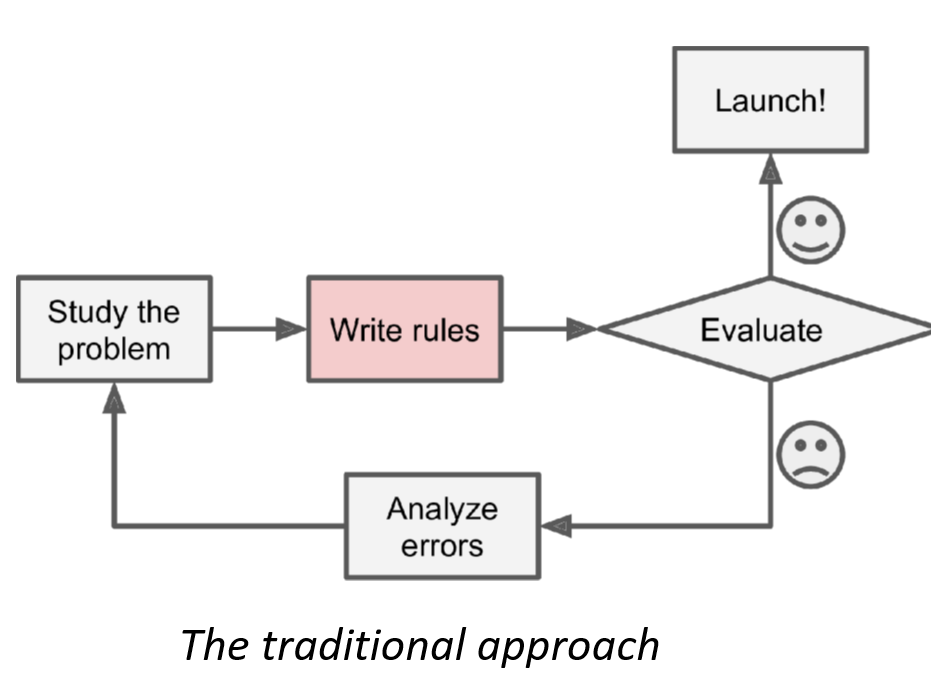
\includegraphics[width=\linewidth]{images/linear-regression/linear-regression-1.png}
        \end{minipage}
        \hfill
        \begin{minipage}{0.48\textwidth}
            \centering
            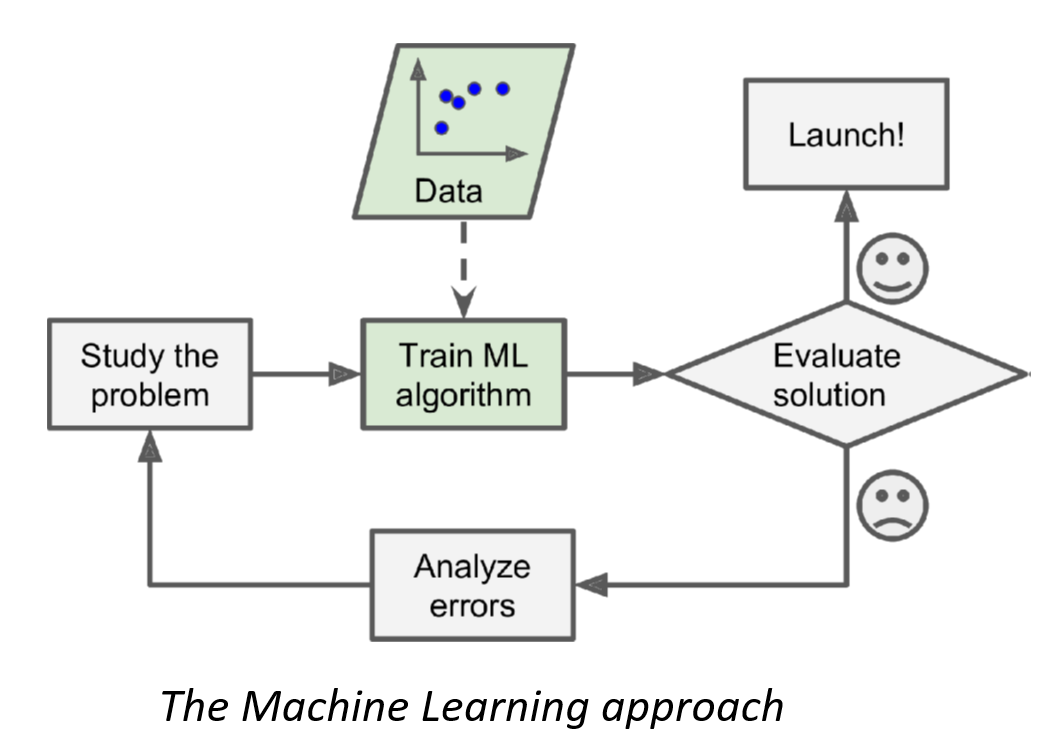
\includegraphics[width=\linewidth]{images/linear-regression/linear-regression-2.png}
        \end{minipage}
    \end{figure}
\end{frame}


\begin{frame}{Data Types}
    \begin{itemize}
        \item \textbf{Tabular Data} (e.g., spreadsheets, databases)
        \begin{itemize}
            \item Note: Columns are called \textbf{Features}. Rows are called \textbf{Samples}.
        \end{itemize}
        
        \item \textbf{Time-Series Data} (e.g., stock prices, weather forecasts, IoT sensor data)
        
        \item \textbf{Text Data} (Natural Language Processing, e.g., emails, social media posts, documents)
        
        \item \textbf{Images and Videos} (Computer Vision, e.g., medical imaging, surveillance, facial recognition)
        
        \item \textbf{Audio Data} (Speech Recognition, Music Processing, e.g., voice commands, podcasts, sound classification)
    \end{itemize}
\end{frame}


\begin{frame}[allowframebreaks]{ML Algorithm Types}
    \begin{itemize}
        \item \textbf{Supervised}: The algorithm learns from labeled data.
        \begin{itemize}
            \item \textbf{Regression}: Predict continuous value (e.g. house prices).
            \item \textbf{Classification}: Predict discrete value (e.g. spam/not-spam).
        \end{itemize}

        \item \textbf{Unsupervised}: The algorithm works on unlabeled data. We are interested in things like:
        \begin{itemize}
            \item \textbf{Clustering}: Grouping
            \item \textbf{Dimensionality Reduction}: Reducing the Dimensions
            \item \textbf{Anomaly Detection}: Detecting outliers
        \end{itemize}

        \item \textbf{Reinforcement Learning}: involves learning to make decisions by interacting with an environment.
        \begin{itemize}
            \item \textbf{Reward Signal}: The agent receives feedback in the form of rewards or penalties, guiding its learning.
            \item \textbf{Policy}: A strategy the agent learns to decide actions based on the current state.
            \item \textbf{Value Function}: An estimate of the expected cumulative reward from a state or state-action pair.
            \item \textbf{Exploration vs Exploitation}: The agent balances exploring new actions to discover rewards and exploiting known actions to maximize them.
            \item Really popular in video games and robotics! (Also recently in LLMs, see \href{https://www.superannotate.com/blog/rlhf-for-llm}{RLHF})
        \end{itemize}
    \end{itemize}
\end{frame}


\begin{frame}{Example: Spam Classification}
    \begin{figure}
        \centering
        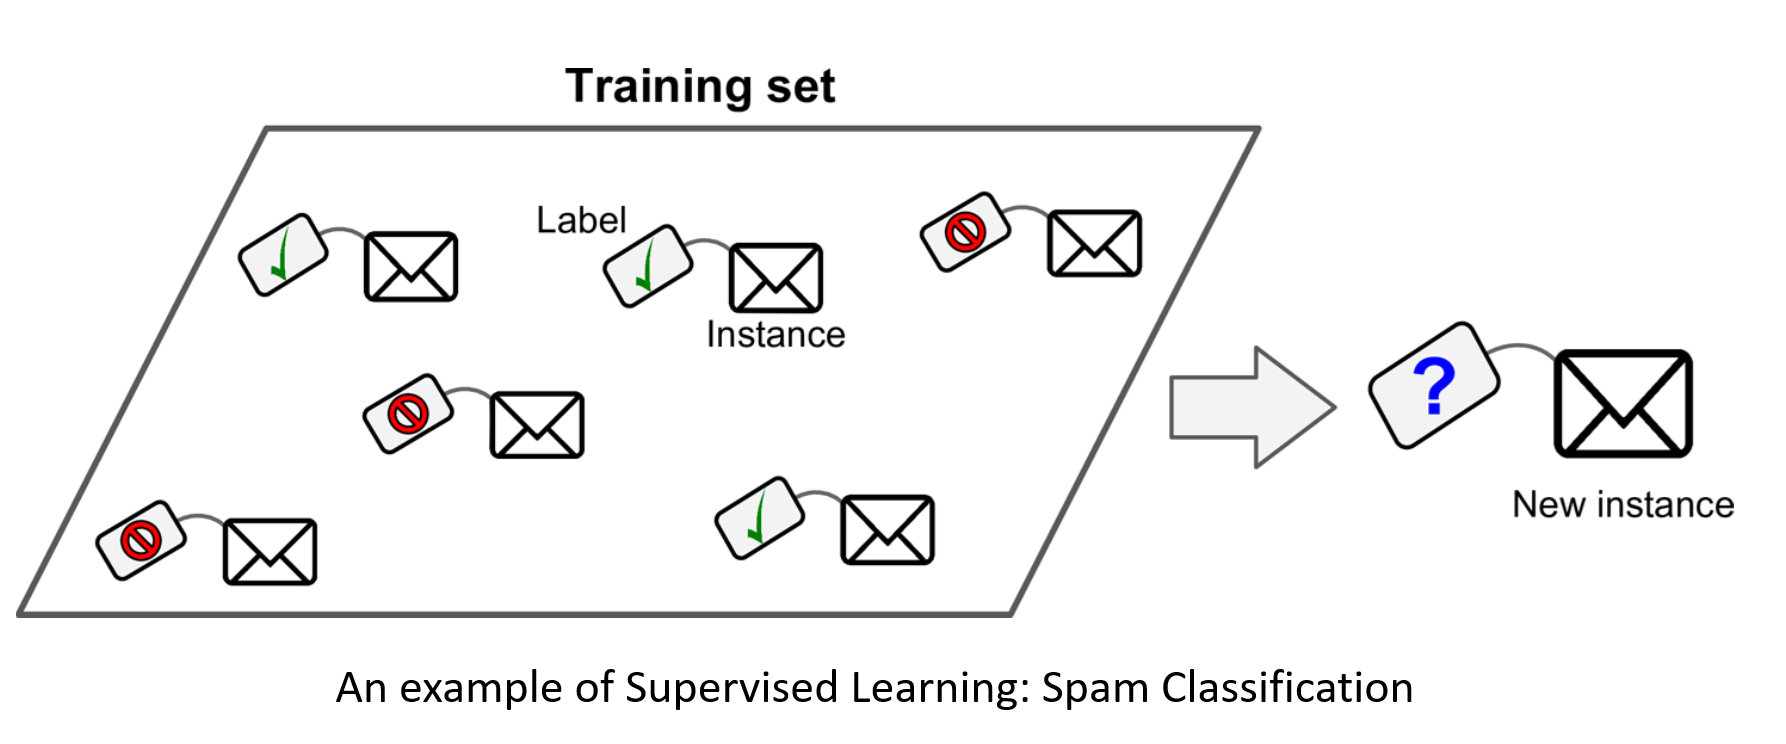
\includegraphics[width=0.85\textwidth]{images/linear-regression/linear-regression-3.png}
    \end{figure}
\end{frame}


\begin{frame}{Example: Clustering}
    \begin{figure}
        \centering
        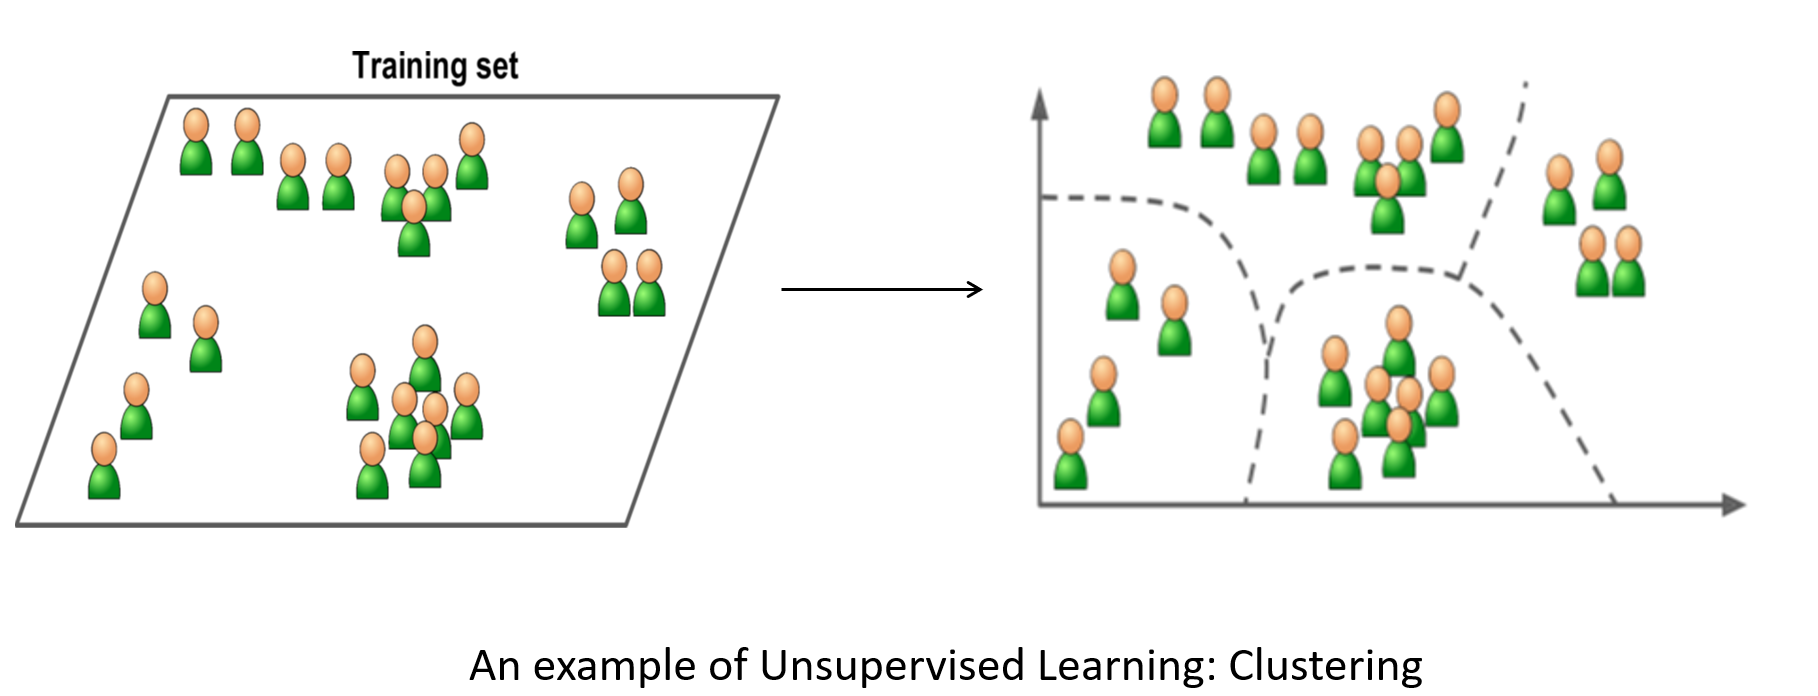
\includegraphics[width=0.85\textwidth]{images/linear-regression/linear-regression-4.png}
    \end{figure}
\end{frame}
